\documentclass[sigconf]{acmart}

\usepackage{booktabs} % For formal tables
\usepackage{paralist} % For compactenum/compactitem


% Copyright
%\setcopyright{none}
%\setcopyright{acmcopyright}
%\setcopyright{acmlicensed}
\setcopyright{rightsretained}
%\setcopyright{usgov}
%\setcopyright{usgovmixed}
%\setcopyright{cagov}
%\setcopyright{cagovmixed}



\copyrightyear{2021}


\begin{document}
\title{Exploring the Impact of Social Influence Mechanisms\\ on Societal Polarization}
%\titlenote{Produces the permission block, and
 % copyright information}
%\subtitle{Extended Abstract}
%\subtitlenote{The full version of the author's guide is available as
 % \texttt{acmart.pdf} document}

\author{Justin Mittereder}
\affiliation{%
  \institution{University of Mary Washington\\Department of Computer Science}
  \streetaddress{1301 College Avenue}
  \city{Fredericksburg}
  \state{Virginia}
  \postcode{22401}
}
\email{jmittere@umw.edu}


% The default list of authors is too long for headers.
\renewcommand{J. Mittereder}

\begin{abstract}
We present an agent-based model, inspired by the opinion dynamics (OD) literature, to explore the underlying behaviors that may induce societal polarization. Our agents interact on a social network, in which adjacent nodes can influence each other, and each agent holds an array of continuous opinion values (on a 0-1 scale) on a number of separate issues. We use two measures as a proxy for the virtual society's ``polarization:'' the average assortativity of the graph with respect to the agents' opinions, and the number of issues on which agents have persistent disagreement even after the model reaches an equilibrium.

We look at two model parameters that affect polarization. The first is the density of edges in the network: this corresponds to the average number of meaningful social connections that agents in a society have. Contrary to our early hypothesis, we find that lower edge density results in higher levels of assortativity. The second is the ``openness'' of agents to differing opinions; \textit{i.e.}, how close a neighboring node's opinion on an issue must be to an agent's own before the agent will adjust its opinion on a different issue. We refer to this novel mechanism as cross-issue influence. Through this mechanism, we find that when agents in the model are less open to new opinions, there will be less consensus on any given issue for all agents in the model.   
\end{abstract}


\ccsdesc[500]{Computing methodologies~Modeling and simulation}
\ccsdesc[500]{Computing methodologies~Agent / discrete models}

\keywords{opinion dynamics, echo-chambers, binary voter model, social networks, polarization}

\maketitle

\section{Introduction}

The recent events that transpired at the U.S.~Capitol on January 6th were a
vivid reminder of the deep divide within the nation. There are signs that the
United States is experiencing political polarization now like it has never seen
before. As individuals stormed the Capitol, Americans watched in horror.
Although this singular event is now in the past, the underlying tension that
preceded it still remains.

Polarization -- reflected in echo chambers, entrenched views, and the
vilification of those whose opinion differs -- can be harmful to a democratic
society. It can inhibit the reaching of consensus and compromise upon which a
democracy is built, and can result in even greater amounts of damage than what
ensued in the U.S.~on January 6th if left unchecked. Further, polarization
affects not only political actors, but also the interpersonal relationships
among the rank and file citizens of a country which bolster and strengthen
society.

In my research, I look at multiple societal variables that I believe may
significantly impact polarization in a society. The first is the density of
social connections: in other words, the average number of social ties a member
of that society has. The second is the degree of ``openness'' in the society:
namely, how willing its members are to consider changing their views. The third is the degree of ``disgust'' in the society: namely, how easily its members are disgusted by opposing views. In addition, I look at two different influence mechanisms. I suspect that these factors play a role in determining the aggregate
polarization of a society.

In order to explore these phenomena, I created an Agent-Based Model (ABM) of
heterogeneous agents in the spirit of much of the Opinion Dynamics (OD)
literature. These agents interact with each other on a random, static social
network and change their opinions on issues over time based on the opinions of
their network neighbors. One novel feature of our model, termed cross-issue influence,
is the way agents influence one another: one agent will not allow another agent to influence its
opinion on an issue (the influence issue) unless the two agents already have sufficient agreement on
another randomly chosen issue (the comparison issue). Additionally, the agent may potentially be repelled away from its neighbor's opinion on the influence issue if the difference in their opinions is far enough away on the comparison issue. The justification for this is related to the
well-known observation of ``homophily'' in social psychology: people are prone
to trust those who already agree with them on something, and hence are more
likely to be persuaded by them on other matters.

The goal of my research is to determine what micro behaviors of individuals
are sufficient to produce a change in the degree of political polarization in
the society. As explained below, we choose to measure polarization in two
different ways: the average similarity of an agent to its neighbors (called
``assortativity'' in social network terminology), and the number of distinct opinion buckets in the society. 
literature).

\section{Topic Introduction}

\subsection{Modeling and Simulation}
First, modeling and simulation is the large field that my research falls under. Modeling and simulation is a rapidly expanding field where the goal is to model an environment to explore phenomena or effects that occur (or will occur) in the real-world. Models can be made to explain or predict real-world behavior. In the field of modeling and simulation, professionals in many disciplines have used methods to simulate complex real-world systems. For example, many people benefit from these types of simulations every day when they check weather applications. Weather apps take in large amounts of data from live feeds in the environment. Then, researchers use the data to create a simulated environment where they can observe and predict future weather outcomes. Another area where this type of model is used is in the predictions of stock prices. Economists are able to input large amounts of data into a model which can predict the direction of stock prices. These types of simulations that are created to be as close to real-world systems as possible are called facsimiles. They are extremely complex and require large amounts of data to retain their predictive power. The models that I wish to do research on are different from these complex and costly models. My goal is not to create a one-to-one model of the United States in 2010 and see if political polarization develops by 2021. This would not be feasible as I would need to model the United States in 2010 which is an impossible task. Instead, I will create a simulation where agents (who represent people) interact on a social network and slowly change the views of those around them in what is called an \textbf{Agent-Based Model}.  

\subsection{Modeling Techniques}
Within the field of modeling and simulation, there are many techniques that have been used to model complex systems. One such technique is discrete event simulation (or DES). In DES, states are modeled as atomic representations of the environment. For example, travel can be modeled with DES. A traveler starts in one location \textit{A}, flys to another location \textit{B}, and then drives to the final location \textit{C}. Another modeling technique is system dynamics (or SD). SD is a more calculus-centered approach. These models are often used to measure continous relationships between entities in fields like industrial economics, environmental policy, and demography.

\subsection{Agent-Based Modeling}
Although DES and SD are useful modeling techniques, they are not applicable for every complex system. These traditional modeling techniques are useful in the aggregate; however, they often fail to capture the impact of agent heterogeneity. For example, macroeconomic models assume that all agents are homogenous which allows for a simpler model. Such models allow for conclusions about the equilibrium conditions of an economy. Although these equilibrium conclusions are helpful for policy decisions, homogenous agents limit the complexity and authenticity of a simulation of human behavior because real people are neither carbon copies of one another, nor totally deterministic in their relationships and choices. Given my research topic of political polarization, a DES or SD model would not be the right approach. The method that I use is \textbf{agent-based modeling} which is commonly called an ABM for agent-based model. ABMs allow agents to have their own behavior according to characteristics that are unique to that particular agent which is extremely beneficial in simulating a social network. \\

Agent-Based modeling is a technique that is growing in popularity. Historically, agent-based modeling has not been a widely used approach in the field of modeling and simulation due to computing power restrictions. Large agent-based models generally suffer from the issues of high space and time complexity. In the past, agent-based models were even simulated by researchers calculating mathematical results by hand without the aid of computer programs. With 21st century technology, we are able to simulate large systems using ABMs of heterogenous agents. 

Some common uses of ABMs are in the study of social and cultural phenomena in economics, demography, and sociology. Additionally, ABMs are used to study natural phenomenon in fields like biology and epidemiology. With the Covid-19 pandemic, the popularity of ABMs have soared due to their ability to model disease transmission through a population where individuals respond differently to policy decisions like lockdowns and mask mandates and to health offerings like vaccines. 

Using an ABM, my aim is "...to 'grow' certain social structures in the computer...the aim being to discover fundamental local or micro mechanisms that are sufficient to \textit{generate} the macroscopic social structures and collective behaviors of interest"(Joshua Epstein in Growing Artificial Societies **need citation). I attempt to discover the micro mechanisms that are sufficient to produce the social and cultural phenomenon of political polarization. I pull from other disciplines such as sociology and physcology for theories of human behavior that I will implement on the micro level. I use various computer science and statistics techniques for implementation and analysis of the macro level phenomena that occur in the model.    

In addition to the large benefit of being able to explore macro level phenomena accurately, ABMs are also a practical approach to modeling due to the simple nature of their code implementation. Those that are familiar with the modern object-oriented programming approach (or OOP) may already see the connection between ABMs and OOP. In OOP, objects have instance variables and functions that are unique to that object. Objects are often contained in data structures (which may even be an instance variable of another class). 

Using OOP, I can create an agent class. The agent class may contain instance variables that are useful in modeling such as the age, wealth, location, and neighbors (other agents in the model) of that particular agent object. These agent objects represent entities that exist within the physical or abstract environment of the model. In my case, the agents will represent people, but its possible for agents to be animals, companies, or biological organisms. Often times, an ABM also has a model class that follows the singleton design pattern. This model class generally contains many agents in a data structure. The encapsulation in OOP greatly aids in the development of a large ABM. With the encapsulation of agent objects in a model object, I am able to create model-level functions that provide high-level insights into the behavior of the agent objects. Using an ABM, I will study the \textbf{opinion dynamics} of an artificial society that interacts on a social network.


\subsection{Opinion Dynamics}
Opinion dynamics is the study of how opinions spread throughout a society. Agent-based models are especially useful for studying opinion dynamics because researchers are able to design agents and tailor their behavior. Researchers are able to test the consequences on a society of specific agent behaviors by studying how opinions flow from agent to agent. In my case, I will be designing agents to follow an influence mechanism. Then, I will observe how opinions flow throughout the society.

\subsection{Modeling Terminology}

\textbf{Parameter Suite} and \textbf{Parameter Sweep}: To get robust results when investigating my hypothesis, I ran parameter suites which are batches of models that are run with the same values for each parameter in the model. With results from a parameter suite, I am able to minimize the impact of randomness and outliers. Another useful modeling technique is the parameter sweep. Parameter sweeps allow me to vary one (or multiple) parameter(s) of the model to see how the output of the simulation varies with the parameter. Parameter sweeps consist of many parameter suites. It is helpful to think of parameter suites like playing a game against an opponent \textit{X} times to find the true outcome of the game. Parameter sweeps are like playing against every opponent \textit{X} times to capture the full impact of varying the opponent on your average outcome when playing the game.

\section{Related work}

\subsection{Opinion Dynamics}

Opinion Dynamics models seek to reproduce the phenomenon of individual agents
forming opinions over time via mutual influence. They allow the researcher to
explore the macro-level patterns that may arise in a society from a set
of simple influence rules defined on the micro-level. For instance, the Binary
Voter Model (BVM), the original and perhaps most influential OD model
(\cite{clifford_model_1973, holley_ergodic_1975}), features a set of
interacting agents, each of which holds a binary opinion. The single influence
rule is that agents periodically change their opinion to match one of their
influencers, chosen at random. Among other things, the model demonstrates that
such a system will always eventually reach uniformity of opinion.

Many researchers (\textit{e.g.}, \cite{ghaderi_opinion_2012,
weisbuch_interacting_2001}) have expanded this idea to model continuous, rather
than discrete, opinions: these are typically expressed as real numbers between
0 and 1. In addition to better capturing the nuance of real-life viewpoints
(which are not usually completely black or white on any issue), continuous
opinions lead naturally to incorporating a form of
\textbf{homophily}\cite{mcpherson_birds_2001} into the model: agents will only
choose to be influenced by agents whose existing opinion is already close to
their own. Termed ``\textbf{bounded confidence}'' (BC) by
\cite{hegselmann_opinion_2002}, this feature can result in non-convergence to
uniformity depending on the value of the threshold agents use to gate
influence.\cite{hegselmann_opinion_2002, deffuant_mixing_2000,
tsang_opinion_2014} The term ``\textbf{clustering}'' (or ``opinion
clustering'') has been used to describe the resulting equilibrium reached by
such models, in which subsets of the agents each converge on a different
opinion value and are henceforth no longer persuadable by other agents.

A smaller number of studies have considered ``\textbf{multidimensional
opinions},'' in which each agent maintains a separate opinion on each of
several different ``issues'' rather than on just one.\footnote{This is to be
carefully distinguished from ``\textbf{opinion vectors},'' which represent an
agent's degree of support for each of several alternatives on the \textit{same}
issue. (See, \textit{e.g.}, \cite{sirbu_opinion_2013}.) Unlike multidimensional
opinions, these opinion vectors are often restricted to be members of a
probability simplex.\\\indent To be concrete about the difference, an agent in
a model with multidimensional opinions might ave a value of .8 for the
``pro-gun control'' issue, .9 for the ``raise the minimum wage'' issue, and .4
for the ``restrict fracking'' issue. By contrast, an agent in a model with
opinion vectors might have a value of .2 for the ``raise taxes to fund
infrastructure'' alternative, .7 for the ``cut military spending to fund
infrastructure'' alternative, and .1 for the ``increase IRS audits to fund
infrastructure'' alternative, all possible solutions to the single ``how to
fund infrastructure'' issue. In the latter case, the options are considered
mutually exclusive and must sum to 1 for any agent.\\\indent (Of course, the
specific real-world examples here are only for illustration; OD models
represent ``issues'' and the ``opinions'' about them completely abstractly.)}
The opinions in a multidimensional setting have been modeled as discrete
(\cite{deffuant_mixing_2000}) or even as boolean variables combined in
arbitrary logic formulas (\cite{van_den_herik_modelling_2019,
cholvy_diffusion_2016}). Oddly, modeling multidimensional opinions as an array
of continuous values is rarely seen. One purpose of using multidimensional
opinions could be to see how an agent's opinions on different issues interact
with one another. This is explored by the boolean expressions in
\cite{van_den_herik_modelling_2019} and \cite{cholvy_diffusion_2016}; in
\cite{deffuant_mixing_2000} the multidimensional opinion for each agent is
instead used merely as an element in a vector space whose (Hamming) distance
from other agents' multidimensional opinions can be computed and compared to a
BC threshold.

With respect to these previous efforts, my model resembles the BVM but gives
the agents continuous, multidimensional opinions. My model also implements BC, but in
a different way than models like \cite{tsang_opinion_2014} do: before accepting
the influence of a fellow agent on an issue, an agent in my model must already
be close in opinion to that agent on a \textit{different} issue. Additionally, agents may be repelled away from each other on a different issue if the difference in their opinions is large enough on another seperate issue. This mechanism I refer to as  
cross-issue influence is meant to mimic a phenomenon of human behavior: if I learn that your viewpoint on
issue A is close to my own, homophily suggests that I will trust you, and I
will therefore be willing to consider your viewpoint on issue B. If I think you do not have a reasonable opinion on issue A, I will move away from you on issue B. To my
knowledge, this mechanism of agent influence has not been previously explored.

\subsection{Polarization}

Polarization can mean different things to different people; I therefore begin
by briefly establishing a dictionary of terms that we will refer back to
throughout this paper.

Arguably the most familiar manifestation of polarization -- which I have termed
``\textbf{diametricity}'' -- is when a group experiences opinions shifting away
from common ground to polar sides, leaving nobody `in the middle' on a specific
issue. Although I do believe that this is a type of polarization that may be occurring, I did not study this flavor of polarization in my research. 

In future research, I hope to study this type of polarization, but I wanted to focus on the types of polarization that I believe pose the greatest threat to society. In my opinion, the majority of American's views are not more diametric than they used to be. Even though certain groups of the population are extreme and pose a threat to democratic processes, the types of polarization that I feel are the most dangerous are described below. 

I use the graph theory term \textbf{assortativity} to represent a second type
of polarization, which is rooted in the tendency that people have to form
connections with people who have similar views. This idea is supported by
\cite{klinkner_red_2005} which focuses on physical proximity breeding
connections, as well as \cite{cholvy_diffusion_2016} which states that we are
more likely to form connections with those that we already are in agreement
with on another issue. The well-known concept of homophily comes into play
here, as studied in \cite{davies_twin_2017} and \cite{taylor_exploring_2018}.
Assortativity is a way to quantify the presence of ``echo chambers'' in a
society, in which people are exposed mostly (or solely) to opinions that
confirm what they already
believe.\cite{dandekar_biased_2013,flaxman_filter_2016}

A third form of polarization is one that can be measured as follows:
how often do opinions on issues result in \textbf{clustering}? For
example, if all individuals had the same belief, there would be one opinion
cluster. However, in a polarized society, there are clusters of opinions for any given issue. In this way, higher clustering in a society represents when individuals are entrenched and no longer willing to change their opinion on a given issue. The mechanism that we use in this paper to calculate the number of opinion clusters will be explained later.

Finally, the last form of polarization that I study in this paper is \textbf{issue alignment}. I define issue alignment as the tendency for people who agree on one issue to also agree on other (unrelated) issues. For example, consider the issues of vaccine mandates, abortion, and gun control. It seems clear to me that these issues are unrelated, yet if I were to know one person's opinion on one of these issues, I believe that I could guess their opinions on the other issues to a high degree of accuracy. Simply, issues that should not be correlated with each other seem to be connected in some way. 

If people generally adhere to an entire suite of opinions, I term that society ``issue aligned'', and claim this is an indication of polarization. 

This phenomenon of issue alignment is not one I have seen studied in the opinion dynamics literature which is why I believe it is so important to understand. I have a few theories as to how issue alignment develops in a society. First, it is possible to me that there is some deep underlying principle to people's value systems that connects seemingly unconnected issues. For example, if an individual believes in personal freedom over everything else, then maybe this influences their decisions on a wide range of issues such as gun control, abortion, and vaccine mandates. However, I do not believe that this is the reason issue alignment occurs. 

Another possible explanation for issue alignment is media outlets. Perhaps a small number of popular media outlets each articulates a set of opinions on various issues. If individuals only hear from their media outlet that they subscribe to, then issue alignment could occur.

A third explanation for issue alignment is that individuals following the well-proven principle of homophily are influenced by their social connections across issues. If they are friends, then homophily and common sense would suggest that agreeing on one issue makes these individuals more likely to be influenced towards each other on another issue. As a result, the individuals develop similar views on issues; thus, resulting in groups that have similar viewpoints on multiple issues that are unrelated. The societal result of this cross-issue influence mechanism is issue alignment.   


\section{Variables}

In this section we define the two important independent variables whose effect
on the model's behavior we seek to discover, and the two dependent variables we
measure at simulation's end.

\subsection{Independent variables}

\subsubsection{Openness}

As mentioned earlier, research shows that \textbf{openness} plays a crucial role in an
individual's ability to relate to others, as well how easily they adopt outside
ideas as their own. To quantify this as a model parameter, we incorporate
openness as a threshold on a continuum from 0 to 1; this threshold is used to
compare agent opinions during their pairwise interactions. Low levels of
openness produce models in which agents only very rarely change their opinions
(namely, only when encountering neighboring agents whose opinion on another
issue is very close to their own). High levels produce models in which agents
eagerly incorporate the opinions of others on almost every interaction.

\subsubsection{Edge probability}

The other parameter represented in our model is the \textit{density} of social
connections. To implement the concept of different degrees of social
connection, we used the Erd\"{o}s-R\'{e}nyi graph generation algorithm to
generate a random graph of connected nodes. With the Erd\"{o}s-R\'{e}nyi graph
generation algorithm, we can specify the \textbf{edge probability} which represents the
probability that there will be an edge between any two given nodes. Using the
edge probability, we can control the density of the resulting graph. As a
result, edge probability directly corresponds to the density of social
connections in our model.    

\subsection{Dependent variables}


\subsubsection{Graph assortativity}

One way we measure the simulated society's polarization is through the
resulting network's ``assortative mixing,'' or simply graph
\textbf{assortativity}. This represents the degree to which an agent's opinions
will have similar values to those of its network neighbors, on average.

The assortativity of a network has a value between $-1$ and 1, where 1
indicates ``perfect assortative mixing'' -- \textit{i.e.}, a situation where
every agent's opinions are identical to each of its graph neighbors'. An
assortativity of 0 indicates that the agents' social connections have no
correlation at all with their opinion values: having a social tie with another
agent does not mean an agent is any more (or less) likely to have opinions
similar to that agent. This will be approximately true when the model is
initialized and before the iterative process begins. (Negative assortativity
values correspond to networks in which an agent is \textit{less} likely to
agree with its network neighbors than with agents in general.)

Assortativity is thus a way to measure the extent to which agents become
surrounded by (only) like-minded agents, and are therefore no longer exposed to
alternative points of view. Since we need to obtain the graph's assortativity
with respect to \textit{multiple} attributes (\textit{i.e.}, the opinions an
agent has on all of the issues), we simply compute the network's assortativity
for each issue separately (as defined in \cite{newman_mixing_2003}, p.5) and
average it over all the issues.

\subsubsection{Opinion clustering}

The second dependent variable of our model is opinion \textbf{clustering}. This
measures how often the opinions that agents have on a given issue fail to
converge to a uniform value, instead remaining bifurcated among two or more
values in perpetuity. Each group of agents who, at simulation's end, have the
same opinion on an issue (within some small tolerance $\epsilon$) are termed an
``opinion cluster'' (a term used by \cite{fotakis_opinion_2016}) on that issue.

For clarity, we refer to any issue on which all agent opinions eventually
converge to the same value as a ``\textbf{uniform issue},'' and any issue that
instead produces opinion clusters as a ``\textbf{clustered issue}.''

One challenge is defining what qualifies as an clustered issue, given that
agent opinions are represented as real numbers that may asymptotically converge
to, but never actually reach, the same value. We use the following mechanism.
To calculate the number of clusters for an issue, we add agents to a cluster
after every step of the model. If the absolute value of the difference between
an agent's opinion and the average opinion of a pre-existing cluster is within
a threshold (0.05), the agent is added to that cluster. If this is not the
case, the agent is added to a new cluster in which it is the first occupant.


\section{Model}

The model is presented using an abbreviated version of the ODD
protocol\cite{grimm_standard_2006}.

\subsection{Purpose}

% Make this compatible with definitions in Polarization lit review

The model simulates interactions on a random social network of agents, each
with an array of continuous, numeric \textbf{opinion} attributes. Its purpose
is to investigate the way in which multiple factors contribute to the emergence of
polarization in the network: the \textbf{edge\_probability}, a value reflecting
the density of social connections in the network; the \textbf{openness} threshold, a
value representing how closely one of an agent's opinions must be to that of a
potential influencer in order to accept influence; the \textbf{disgust} threshold, a value representing how far away one of an agent's opinions must be to that of a potential influencer in order to be repelled away on an issue; and the presence of agents following the cross-issue influence mechanism or the same-issue influence mechanism. (See
Section~\ref{modelProcess}, below.)

Using the model, we hope to gain general insight on the emergence of this
polarization within social networks and how different parameters affect this.

\subsection{Entities, State Variables and Scales}

The entities within the model are Agents, having the following attributes:

\begin{description}
\item[ID] A unique ID for the agent.
\item[Opinions] An array of numbers, representing opinions on issues, each
having a value between 0 and 1. This represents the degree to which the agent
``agrees'' or ``disagrees'' with an issue, with 0.5 being neutral.
\item[Neighbors] A subset of the other agents in the model, to whom this Agent
has a social connection. The entire set of Agents and their social connections
form an undirected graph (\textit{i.e.}, all social connections are
bidirectional) and the graph is fixed throughout the simulation.

\end{description}


\subsection{Process Overview and Scheduling}
\label{modelProcess}

After the model has been initialized, the following sequence is executed for
each of a fixed number of steps in the simulation for cross-issue influence agents:

\begin{compactenum}
\item An agent $X$ is chosen at random.  
\item A neighbor of $X$ (call it $Y$) is chosen at random.
\item An issue $I_1$ is chosen at random.
\item The absolute difference between $X$'s opinion on $I_1$ and Y's opinion on
$I_1$ is measured.
\item Another opinion $I_2$ ($\neq I_1$) is chosen at random.
\item If the difference between $X$'s and $Y$'s opinion on issue $I_1$ is less
than or equal to the model's \textbf{openness} threshold, set $X$'s opinion on
$I_2$ to be the average of $X$'s and $Y$'s current $I_2$ opinions.
\item If the difference between $X$'s and $Y$'s opinion on issue $I_1$ is greater
than or equal to the model's \textbf{disgust} threshold, set $X$'s opinion on
$I_2$ to be the difference between $X$'s opinion and the average of $X$'s and $Y$'s current $I_2$ opinions plus $X$'s previous opinion. Note that in this case, $X$'s opinion will move away from $Y$'s on $I_2$. \\ 
\end{compactenum} 

For same-issue influence agents, the following sequence is executed:
\begin{compactenum}
\item An agent $X$ is chosen at random.  
\item A neighbor of $X$ (call it $Y$) is chosen at random.
\item An issue $I_1$ is chosen at random.
\item The absolute difference between $X$'s opinion on $I_1$ and Y's opinion on
$I_1$ is measured.
\item If the difference between $X$'s and $Y$'s opinion on issue $I_1$ is less
than or equal to the model's \textbf{openness} threshold, set $X$'s opinion on
$I_1$ to be the average of $X$'s and $Y$'s current $I_1$ opinions.
\item If the difference between $X$'s and $Y$'s opinion on issue $I_1$ is greater
than or equal to the model's \textbf{disgust} threshold, set $X$'s opinion on
$I_1$ to be the difference between $X$'s opinion and the average of $X$'s and $Y$'s current $I_1$ opinions plus $X$'s previous opinion. Note that in this case, $X$'s opinion will move away from $Y$'s on $I_1$. 
\end{compactenum}

\subsection{Initialization}

The simulation is initialized with 100 agents, each having a variable number of opinions set to
independent uniform random values between 0 and 1. The model is initialized with all agents either following the cross-issue influence mechanism or the same-issue influence mechanism. The agents are then
connected to each other using a random undirected Erd\"{o}s-R\'{e}nyi
graph\cite{erdos_random_1959} with parameters\ $N=100,
p=\textbf{edge\_probability}$. If the graph is not connected, a new random
graph is generated until a connected one is obtained.

An openness threshold and disgust threshold, each having a value between 0 and 1, will be set such that the openness threshold is always less than the disgust threshold.

The model's step limit is usually set to 1000, as most change in the agent's
opinions after 1000 steps is negligible.


\section{Hypothesis}
I form the following hypotheses about the model's behavior.

\textbf{Hypothesis 1a}: ($H_{1a}$). Mean assortativity will increase with the
edge probability of an Erd\"{o}s-R\'{e}nyi graph.

\textbf{Hypothesis 1b}: ($H_{1b}$). Mean assortativity will increase when the
openness threshold of agents in the model is lower.

\textbf{Hypothesis 2a}: ($H_{2a}$). The number of clustered issues will be
negatively correlated with the edge probability of an Erd\"{o}s-R\'{e}nyi
graph.

\textbf{Hypothesis 2b}: ($H_{2b}$). The number of clustered issues will
increase when the openness threshold is lower for all agents in the model.

\textbf{Hypothesis 3a}: ($H_{3a}$). The number of distinct opinion buckets will
decrease when the agents in the model follow the cross-issue influence mechanism compared to same-issue influence mechanism.


For $H_{1a}$, I hypothesize that increasing the connectivity of an
Erd\"o{s}-R\'{e}nyi graph by raising the edge probability will result in higher
assortativity. This hypothesis is based mainly on real-world observations: the
number of social connections available to those with Internet access has
increased in the past few decades (due to social media\cite{dean_how_2021}),
and the degree of homophily exhibited in members of a social circle has also
(at least anecdotally) increased. Since both the density of connections and the
homophily of those joined by such connections has increased in the real world,
I presume the same effect will follow in my model.

For $H_{1b}$, I hypothesize that when agents in the model are less open to new
opinions, there will be a higher average assortativity and therefore
polarization. When all agents have a lower level of openness, they will only be
interacting with agents that have opinions similar to their own; therefore, I
expect to see higher levels of assortativity. 

For $H_{2a}$, I assume that raising the connectivity of an Erd\"o{s}-R\'{e}nyi
graph by increasing the edge probability will result in fewer clustered issues.
As a graph becomes more densely connected, agents will have a wider variety of
neighbors to receive influence from. As a result, agents should merge to the
consensus opinion for any given issue more often in a more densely connected
graph. 

For $H_{2b}$, I believe that lowering the openness threshold of agents in the
model will result in more clustered issues across the model. When agents are
less open to distant opinions, there will be more variety of opinion for any
given issue. 

For $H_{3a}$, I believe that when agents follow the cross-issue influence mechanism, there will be fewer opinion buckets because agents will converge to a few distinct sets of opinions. With the same-issue influence mechanism, there will be less convergence to sets of opinions, and therefore more distinct opinion buckets. 
\section{Results}
\subsection{$H_{1a}$ and $H_{1b}$}

To test $H_{1a}$, we first establish a model with 50 agents, 5 issues, and an
openness parameter of 0.40. In order to measure the impact of varying edge
probability on average assortativity across all issues, we run each combination
of parameters 20 times starting with an edge probability of 0.05 and ending
with an edge probability of 0.95, in increments of .05. The results of this
model run are shown in Figure~\ref{H1a_plot}.

\begin{figure}
\centering
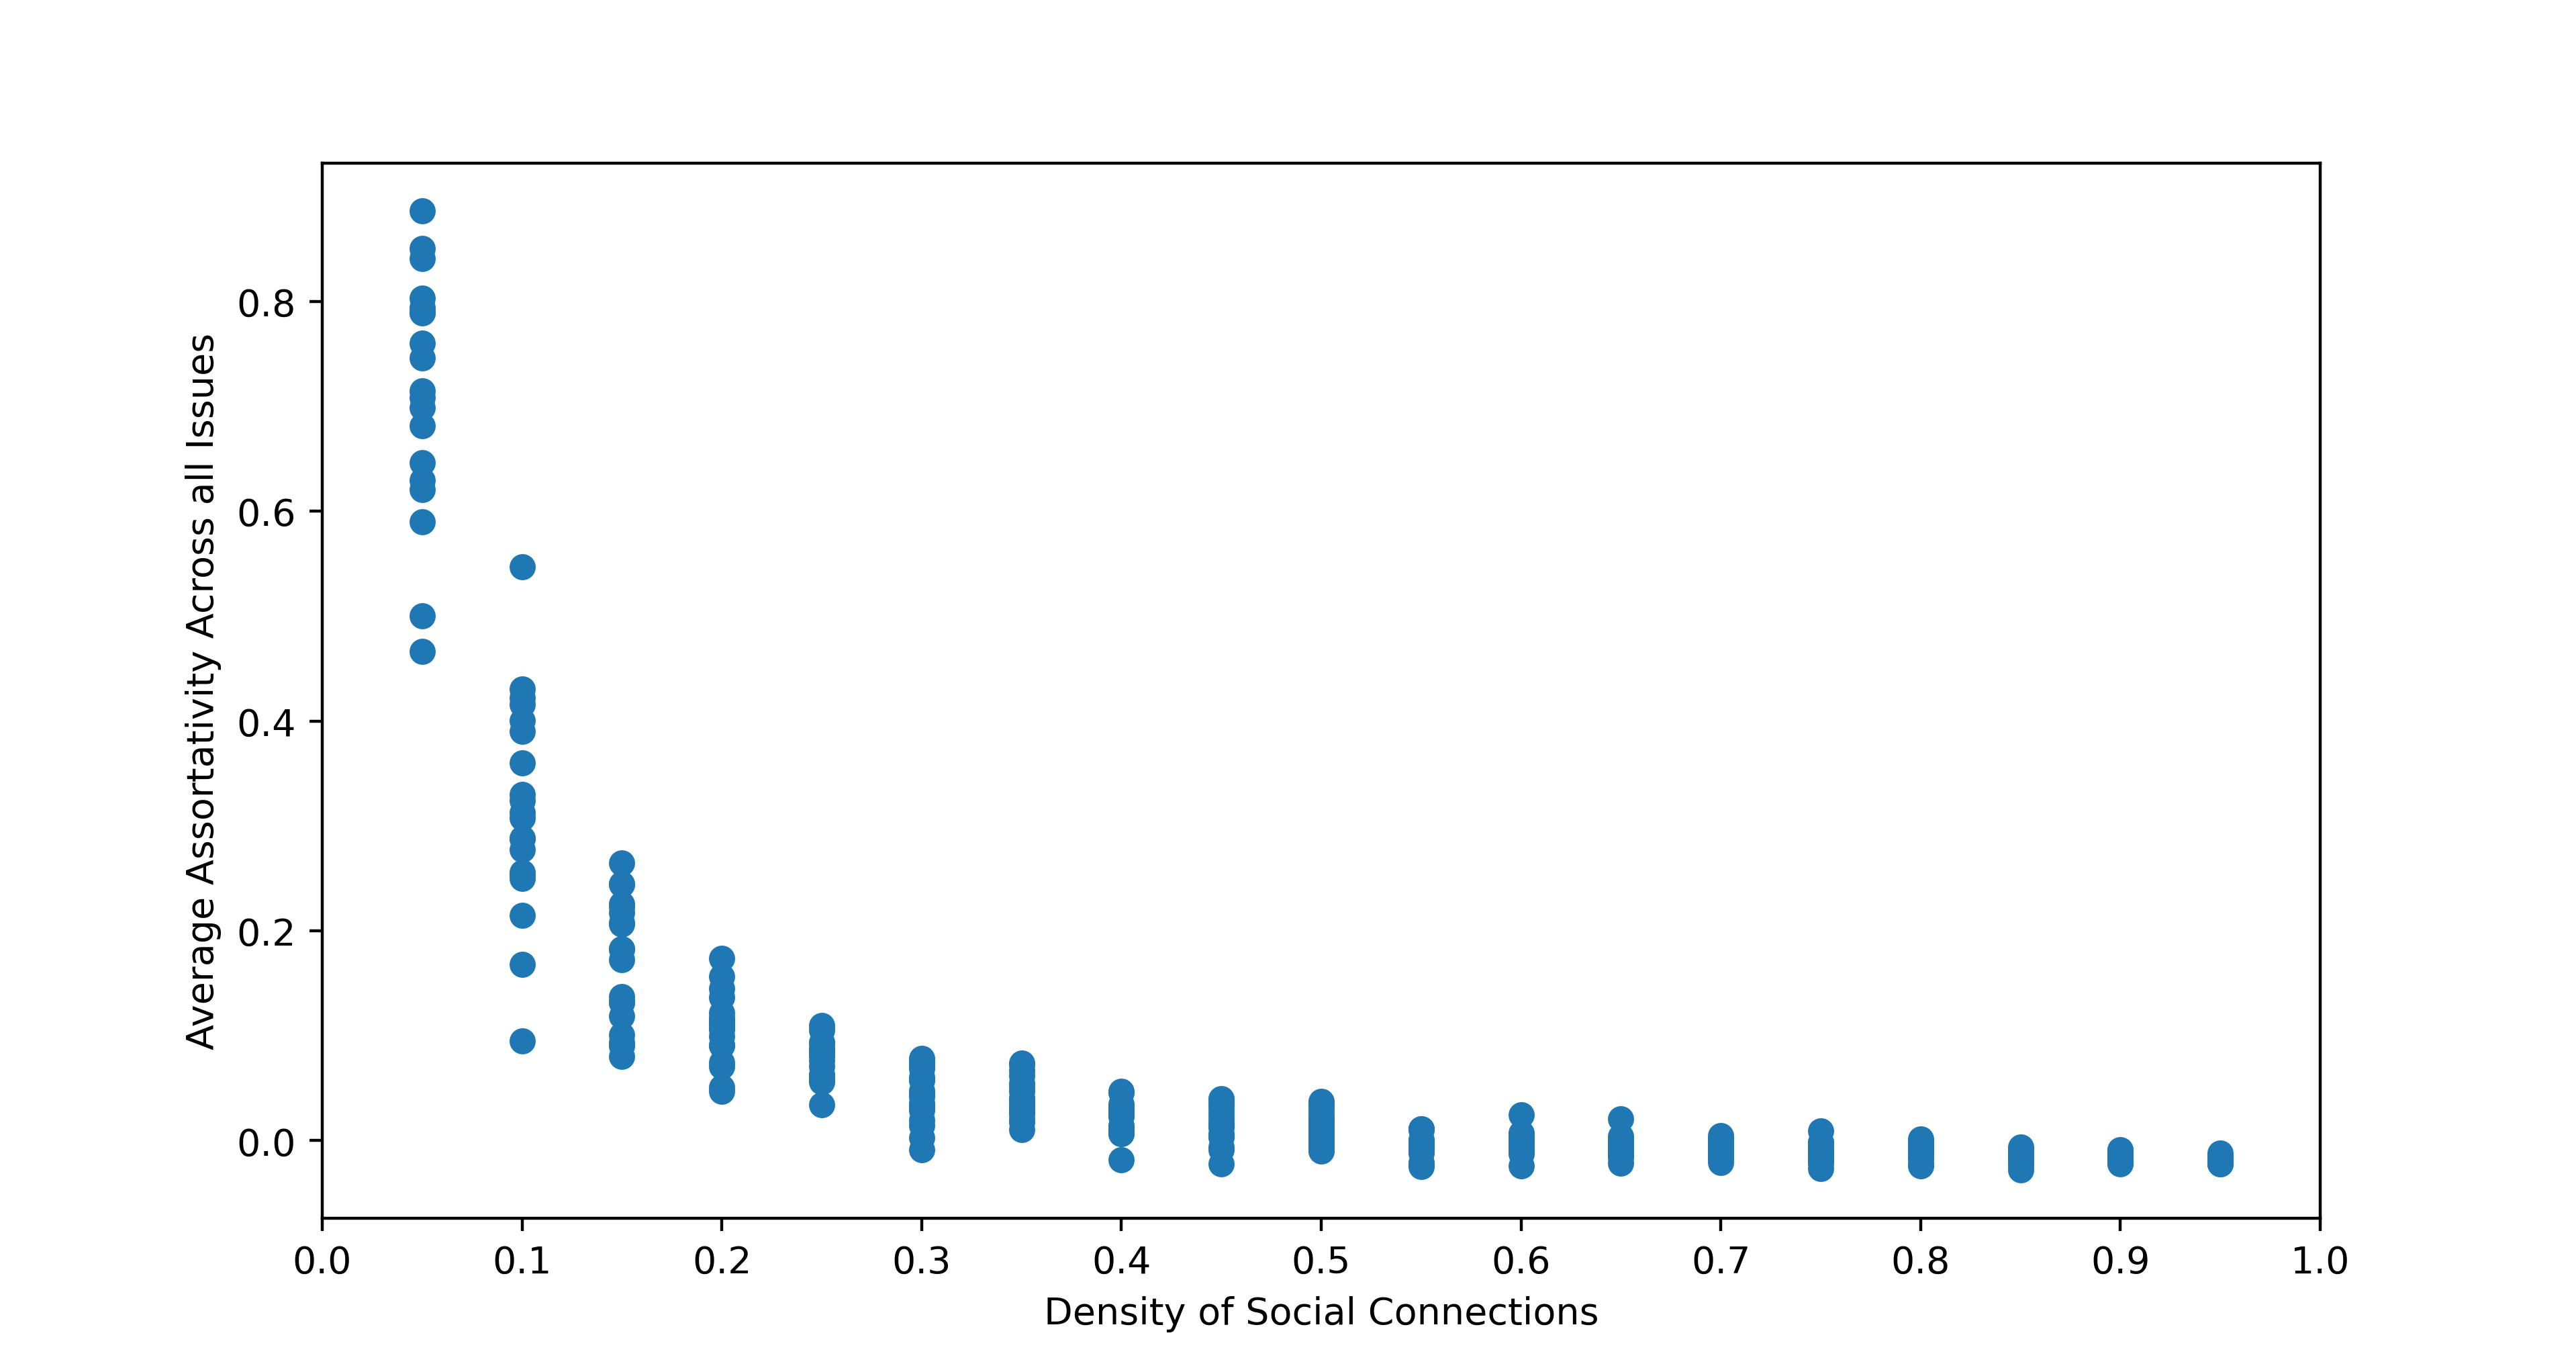
\includegraphics[width=1.0\columnwidth]{./Graphs/Assort_edge.png}
\caption{Average Assortativity across all Issues and Edge Probability}
\label{H1a_plot}
\end{figure}

We see that as the edge probability (or density of social connections)
increases, the average assortativity across all issues decreases. This is the
exact opposite of our hypothesis. One possible explanation for this result is
that when connections are more dense, there is a higher chance that agents will
be exposed to a more diverse set of opinions. There is thus a higher chance
that agents will be pulled to the `average` opinion for a given issue, which
would produce lower assortativity. From this finding, we may be able to infer
that societies where individuals are more densely connected may experience
less polarization than more sparsely-connected societies do.

In addition to the negative correlation between density of social connections
and polarization, we also see that the relationship between these two variables
appears negative-exponential in nature. The variance was too high, however, for
us to draw a solid conclusion on whether the relationship truly conforms to a
negative-exponential, a power-law, or any other standard distribution.

To test $H_{1b}$, we first establish a model with 50 agents, 5 issues, and an
edge probability of 0.50. In order to measure the impact of varying the
openness parameter on average assortativity across all issues, we ran each
combination of inputs 20 times with an openness parameter ranging from 0.05 to
0.95 in increments of .05. The results of this model run are shown in
Figure~\ref{H1b_plot}. As is depicted, there is no obvious relationship at all
between the openness parameter and the average assortativity across all issues. 

\begin{figure}
\centering
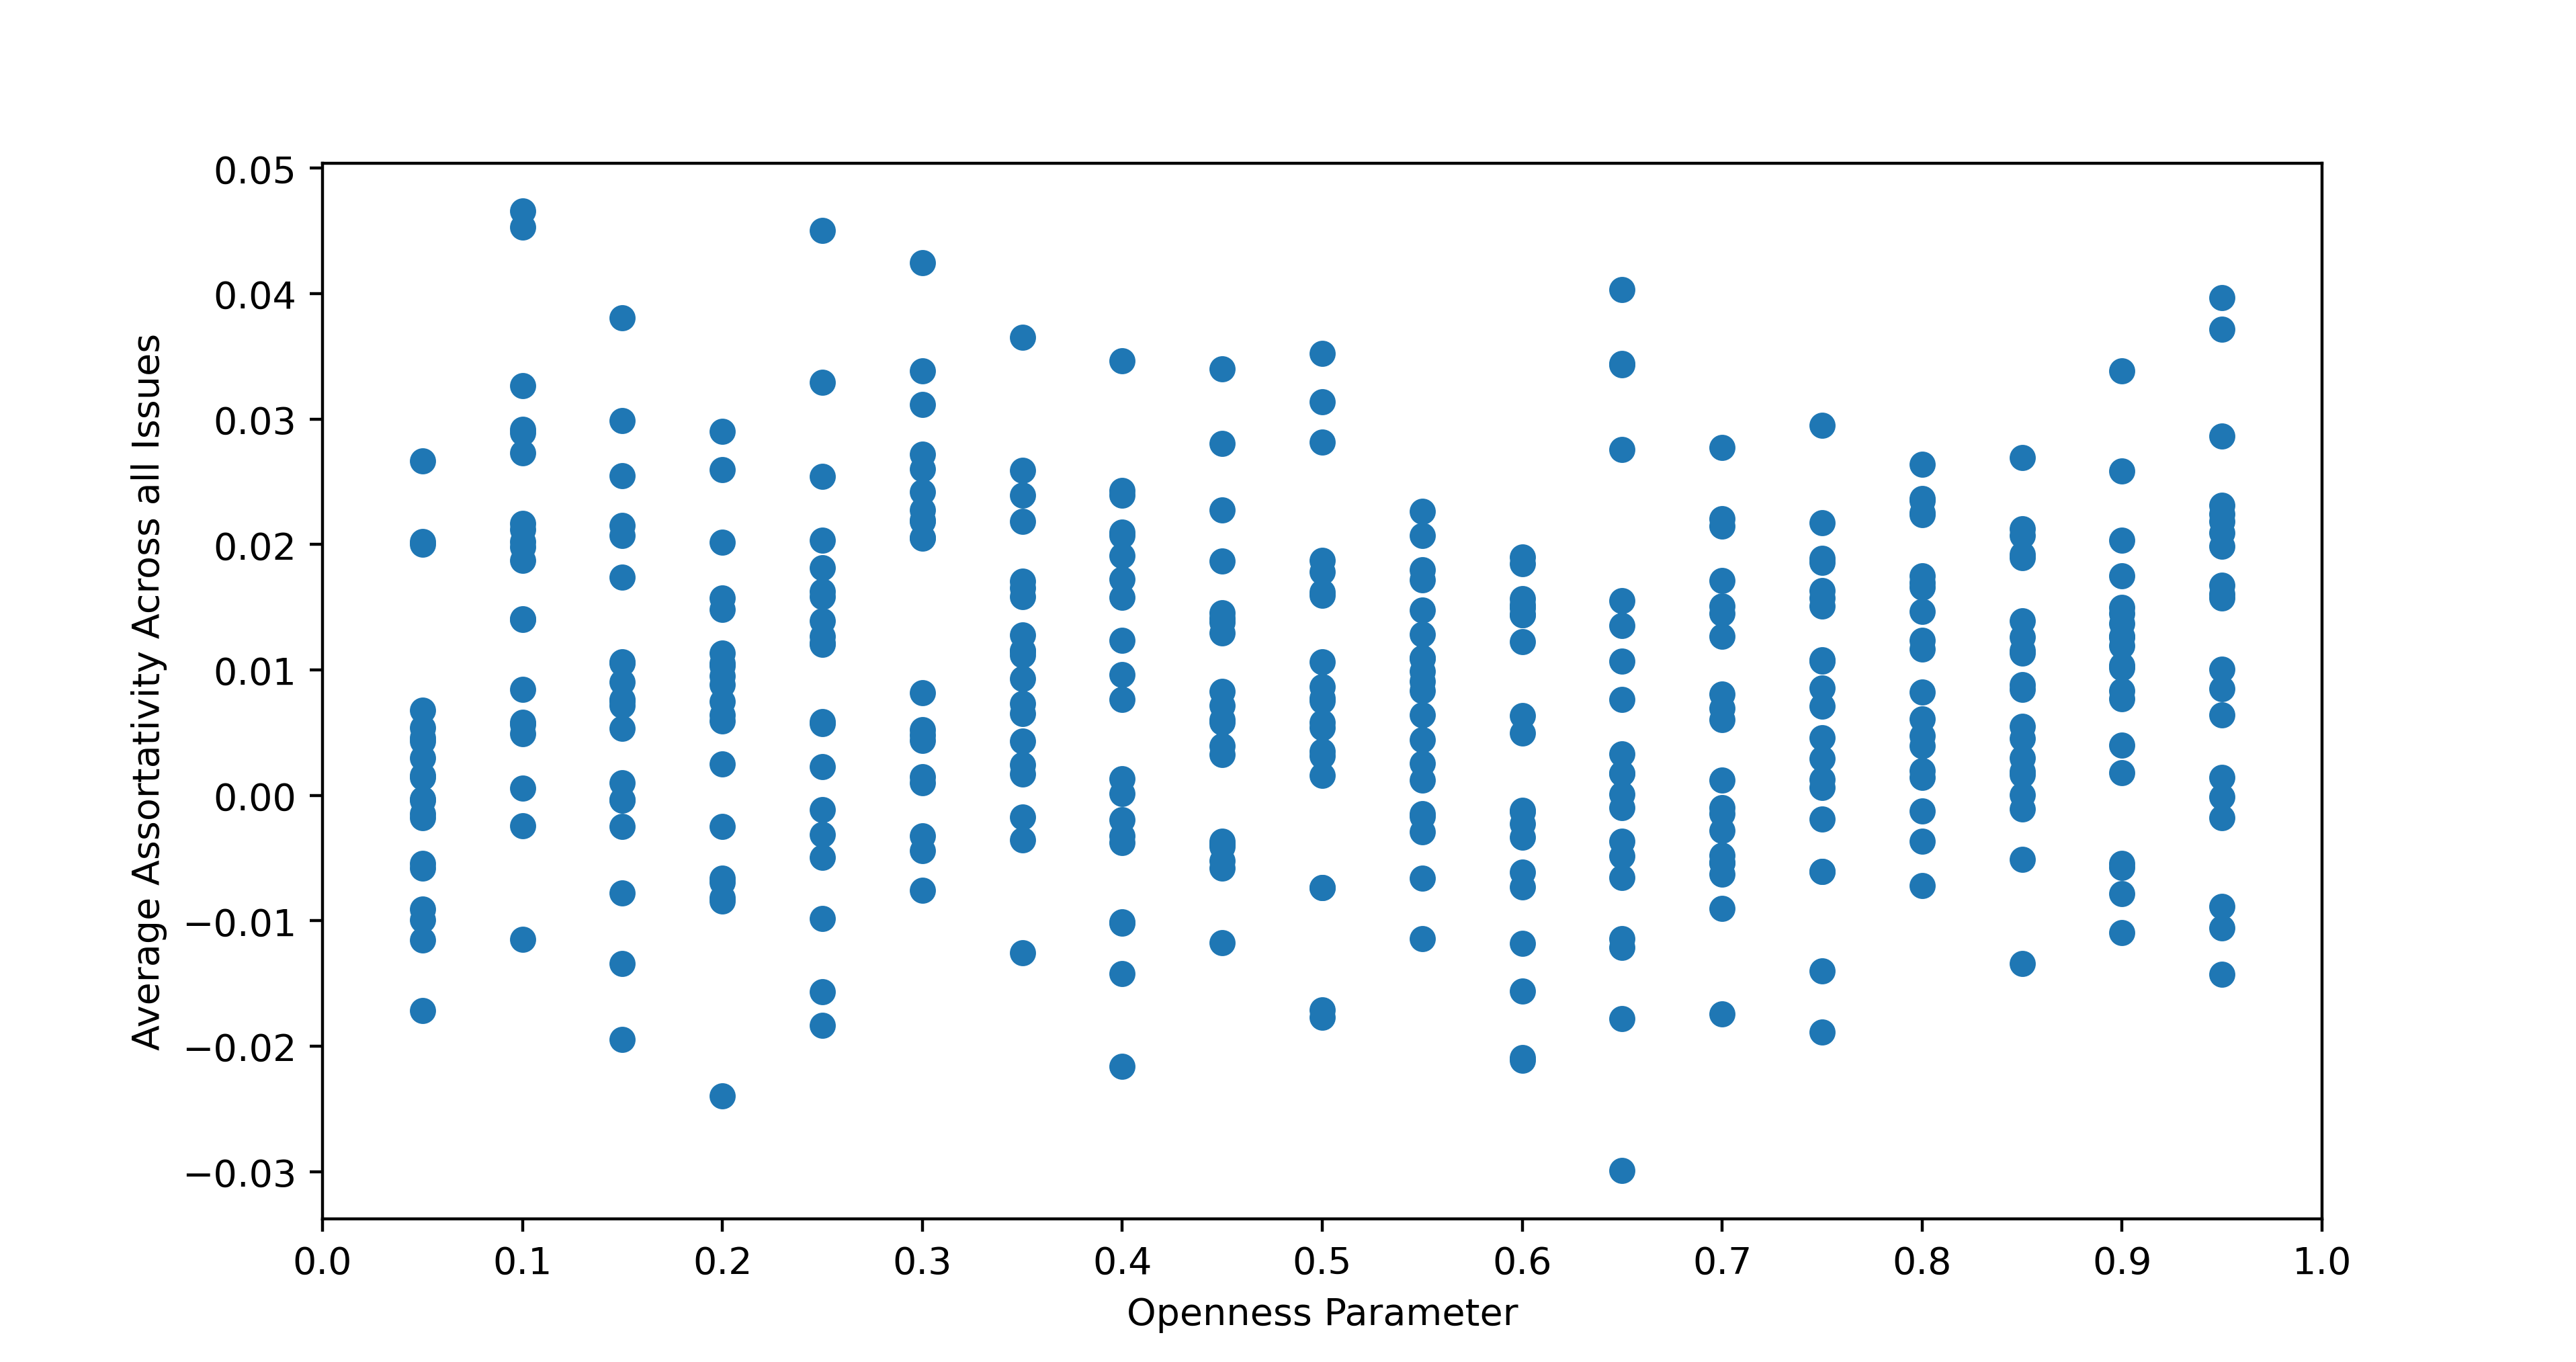
\includegraphics[width=1.0\columnwidth]{./Graphs/Assort_openness.png}
\caption{Average Assortativity across all Issues and Openness Parameter}
\label{H1b_plot}
\end{figure}

This is an interesting result. Agents in the model are influenced when they are
close in opinion (within our openness parameter) to another agent on the same
issue. Therefore, we believed that openness would play a role in determining the assortativity of a society. 
It should be noted that we tested this hypothesis with multiple different values of the edge probability (0.15,
0.40, and 0.50), to ensure that the edge probability was not having an impact
on our results. Even still, we hope to investigate this hypothesis further in future research. 

\subsection{$H_{2a}$ and $H_{2b}$}

To test $H_{2a}$, we establish a model with 50 agents, 5 issues, and an
openness parameter of 0.30. First, we ran a parameter sweep varying the edge
probability from 0.05 to 0.95 to measure the impact of this parameter on the
number of opinion clusters. The results of this parameter sweep are shown in
Figure~\ref{H2a_plot_big}.

\begin{figure}
\centering
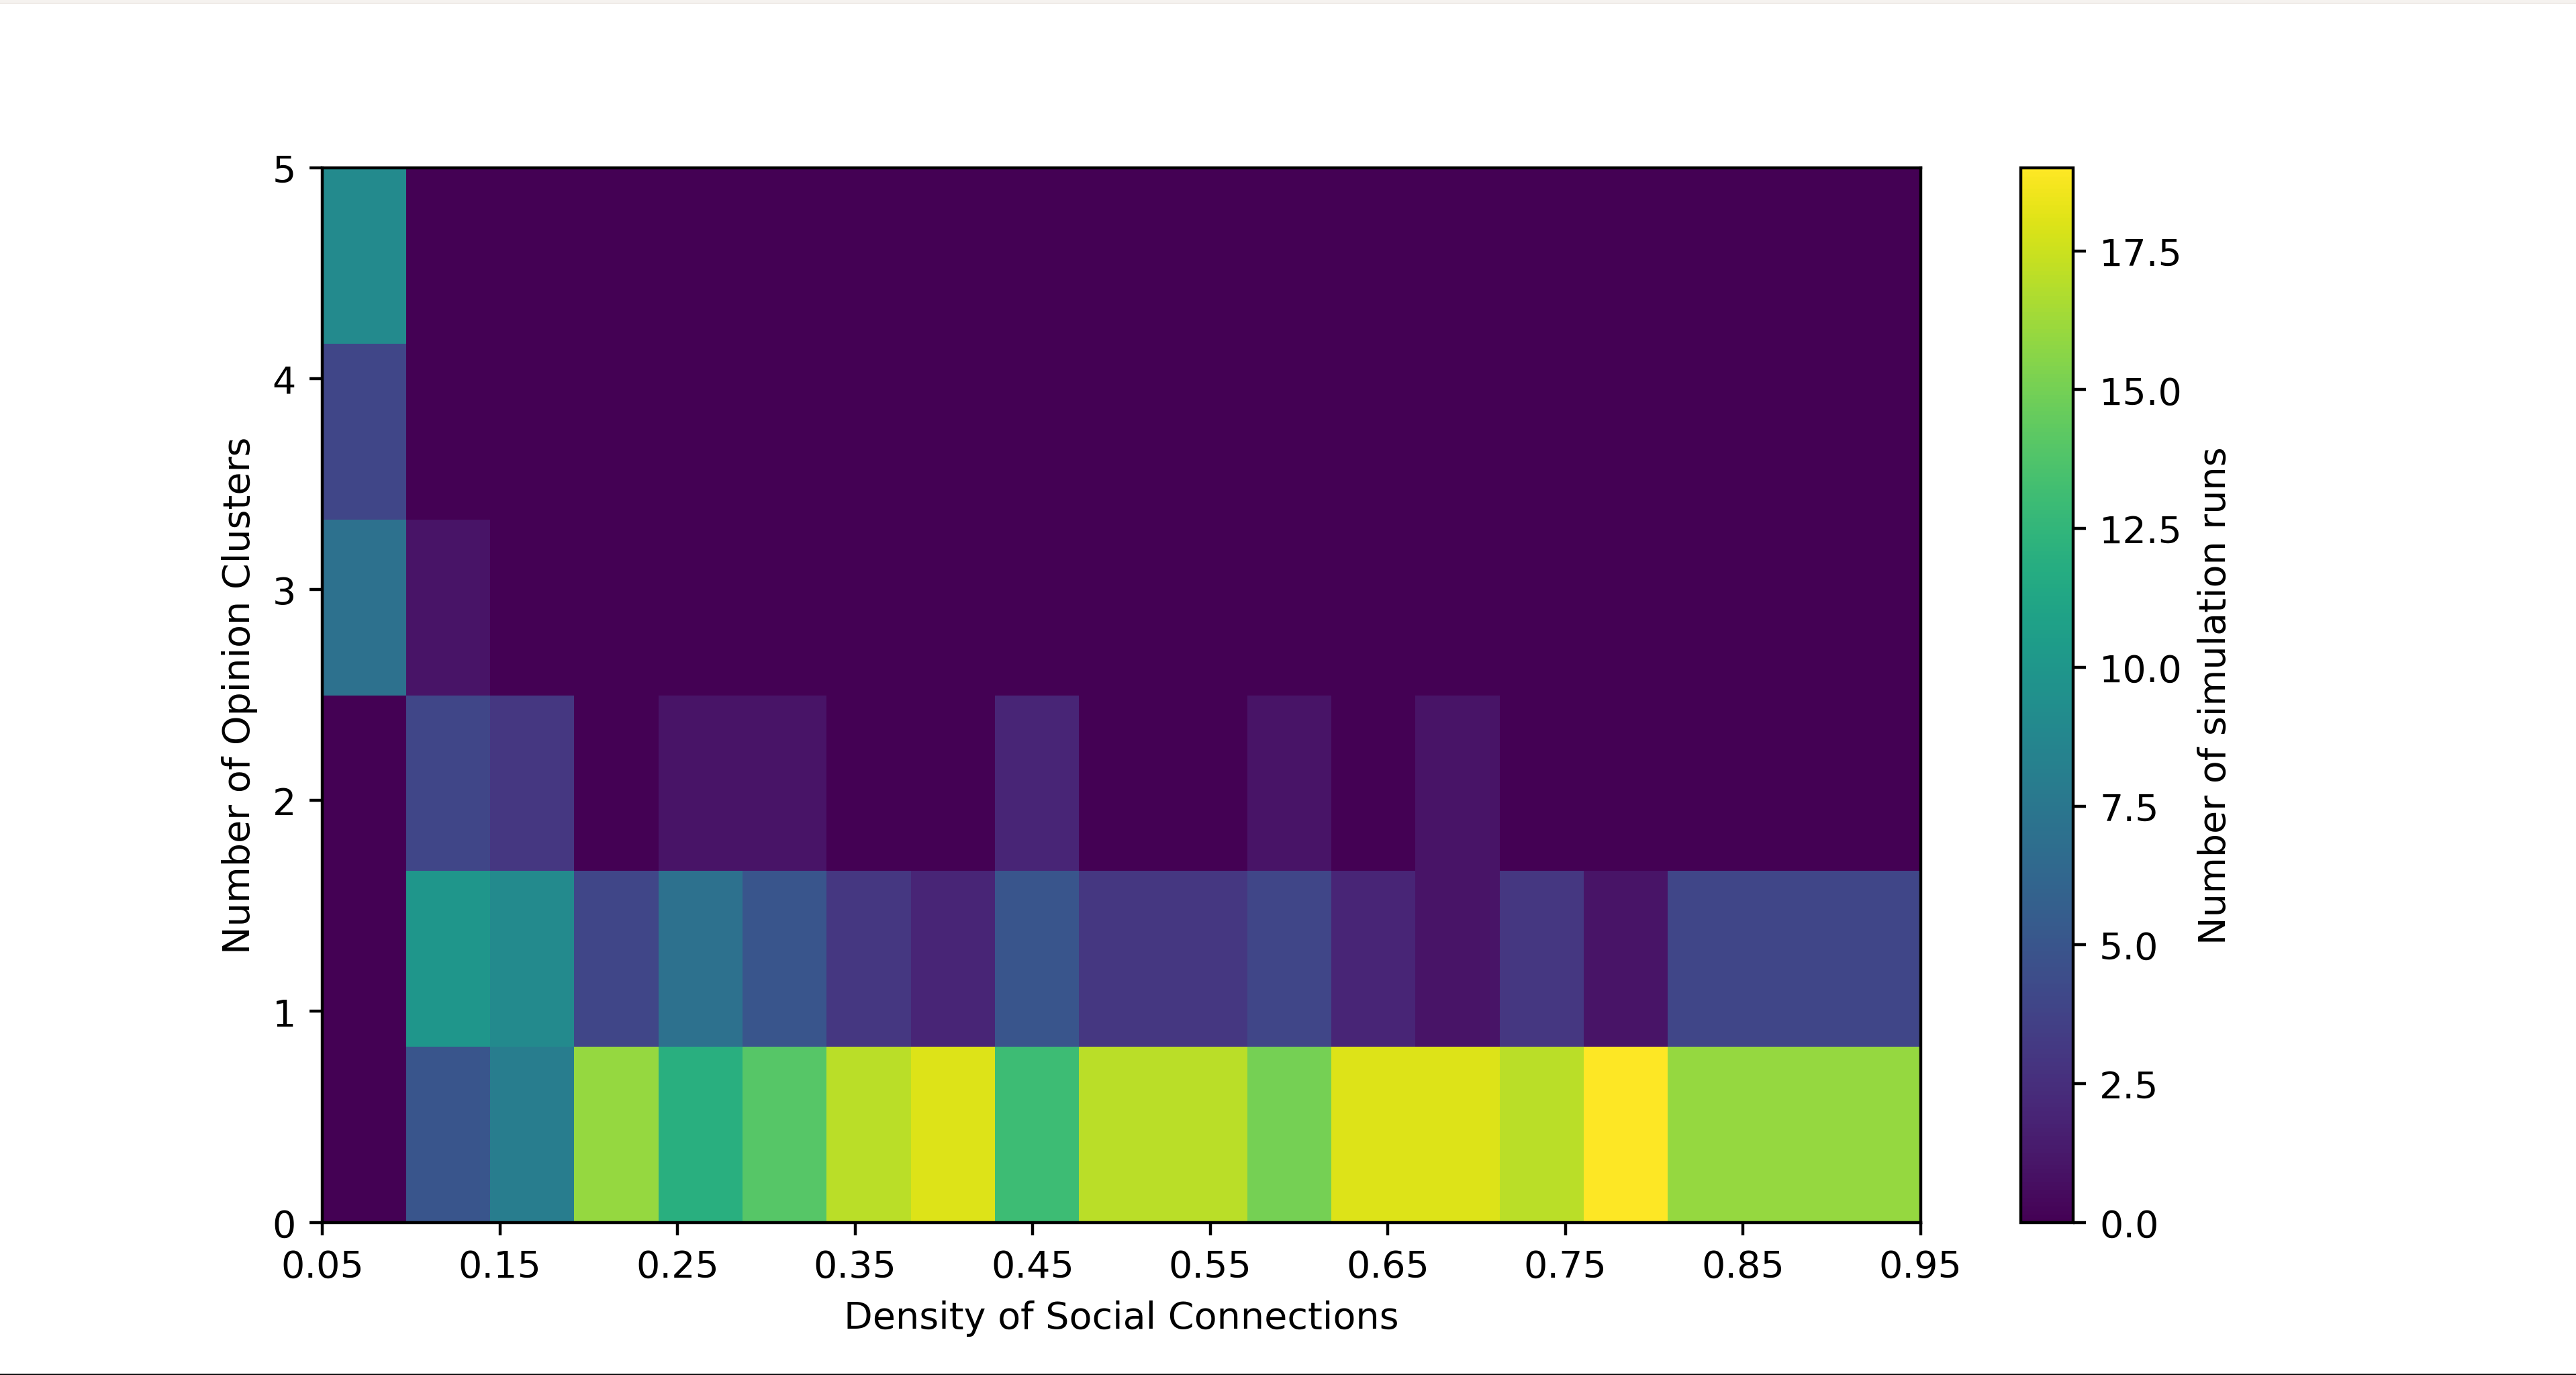
\includegraphics[width=1.0\columnwidth]{./Graphs/ClusterEdge/Cluster_edgeBig.png}
\caption{Number of Opinion Clusters and Edge Probability (0.05 - 0.95)}
\label{H2a_plot_big}
\end{figure}

We noticed that as with $H_{2a}$, there appears to be a tipping point with the
number of opinion clusters and the edge probability. To further explore this
hypothesis, we ran another parameter sweep, this time varying the edge
probability from 0.05 to 0.40 incrementing by 0.01 for each suite of 20 model
runs. The results of this parameter sweep are depicted in
Figure~\ref{H2a_plot_small}.

\begin{figure}
\centering
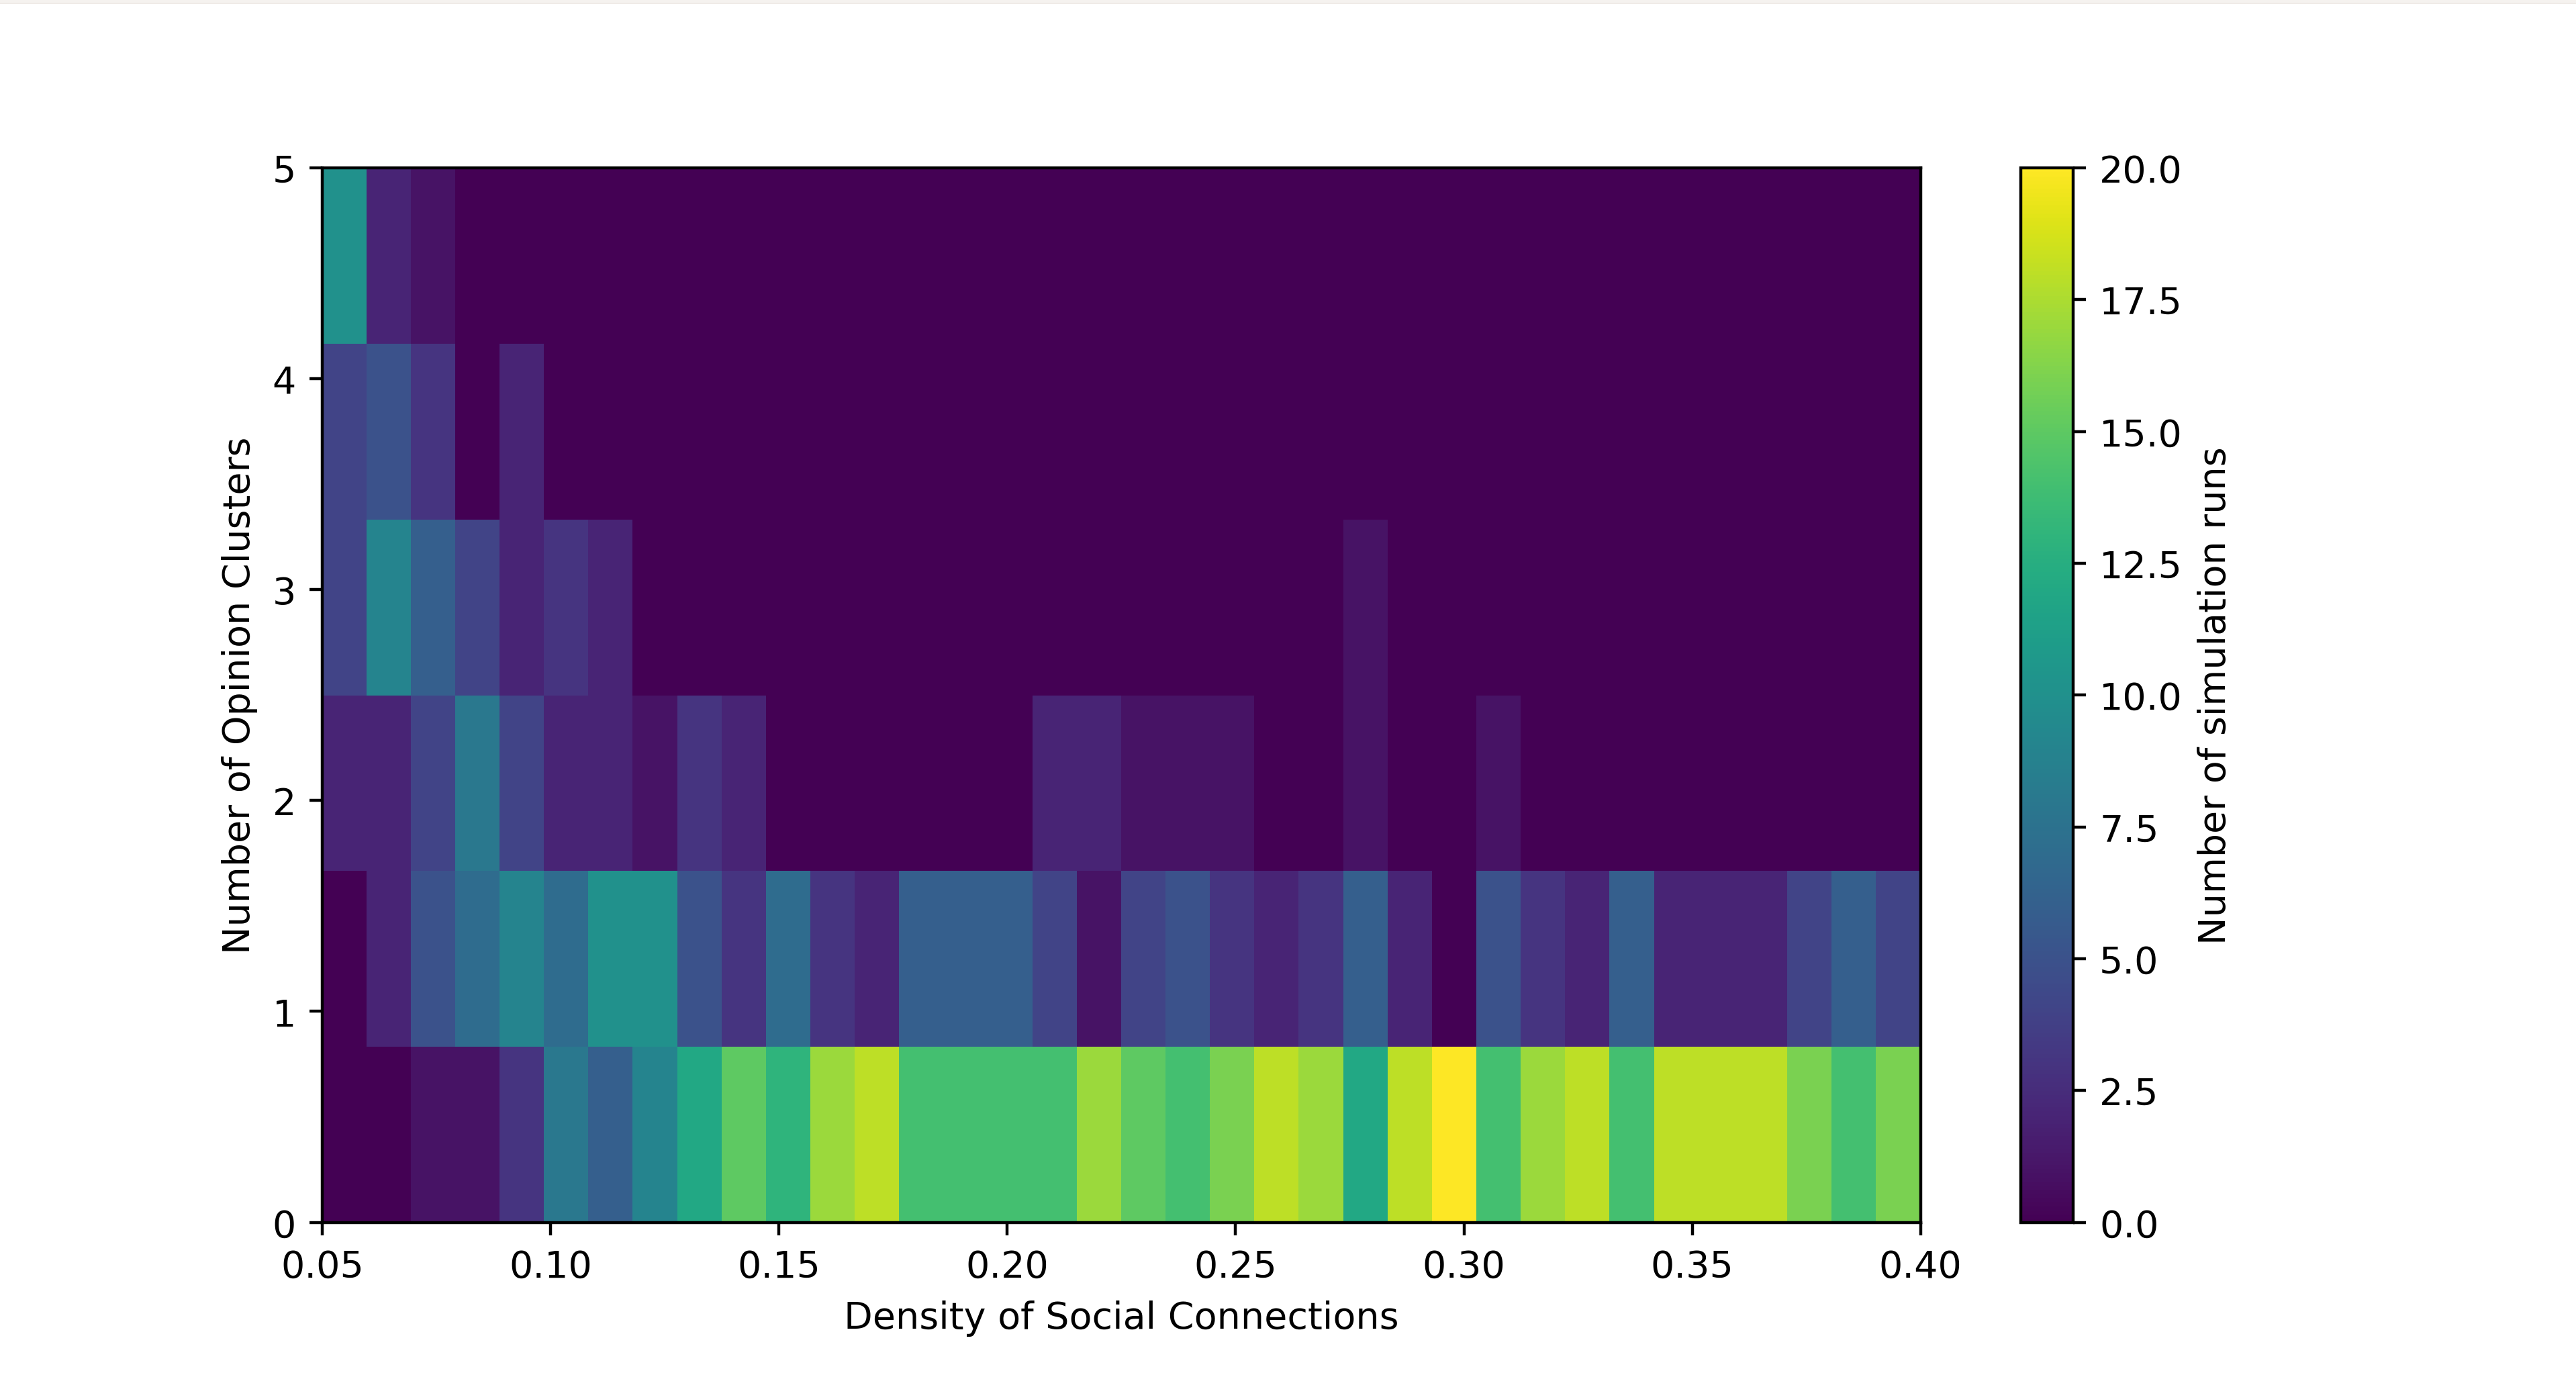
\includegraphics[width=1.0\columnwidth]{./Graphs/ClusterEdge/Cluster_edgesmall.png}
\caption{Number of Opinion Clusters and Edge Probability (0.05 - 0.40)}
\label{H2a_plot_small}
\end{figure}

Our results confirm $H_{2a}$; the number of opinion clusters and edge probability have a negative relationship. We believe this may be explained by the implications of a high density for a graph of nodes. For example, when a graph of 50 nodes has a density of 0.05, the average number of social connections will be 2.5. We are able to calculate the average number of social connections by multiplying the chance there will be an edge between any two nodes (edge probability) and the number of nodes. When the edge probability, or density of the graph, increases slightly to 0.2, the average number of social connections will rise to 10 connections. As a result, the geodesic distance between two nodes decreases rapidly because each node is proportionately connected to more nodes in the graph. This may reveal why we saw that only a certain level of density is required for the number of opinion clusters to drop sharply. Undeniably, a tipping point exists with the number of opinon clusters when increasing the density of an Erd\"{o}s-R\'{e}nyi graph in our model.  

To test $H_{2b}$, we establish a model with 50 agents, 5 issues, and an edge
probability of 0.50. First, we ran a parameter sweep varying the openness
parameter from 0.05 to 0.95 to measure the impact of varying the openness
parameter on the number of opinion clusters. The results of this parameter
sweep are shown in Figure~\ref{H2b_plot_big}.

\begin{figure}
\centering
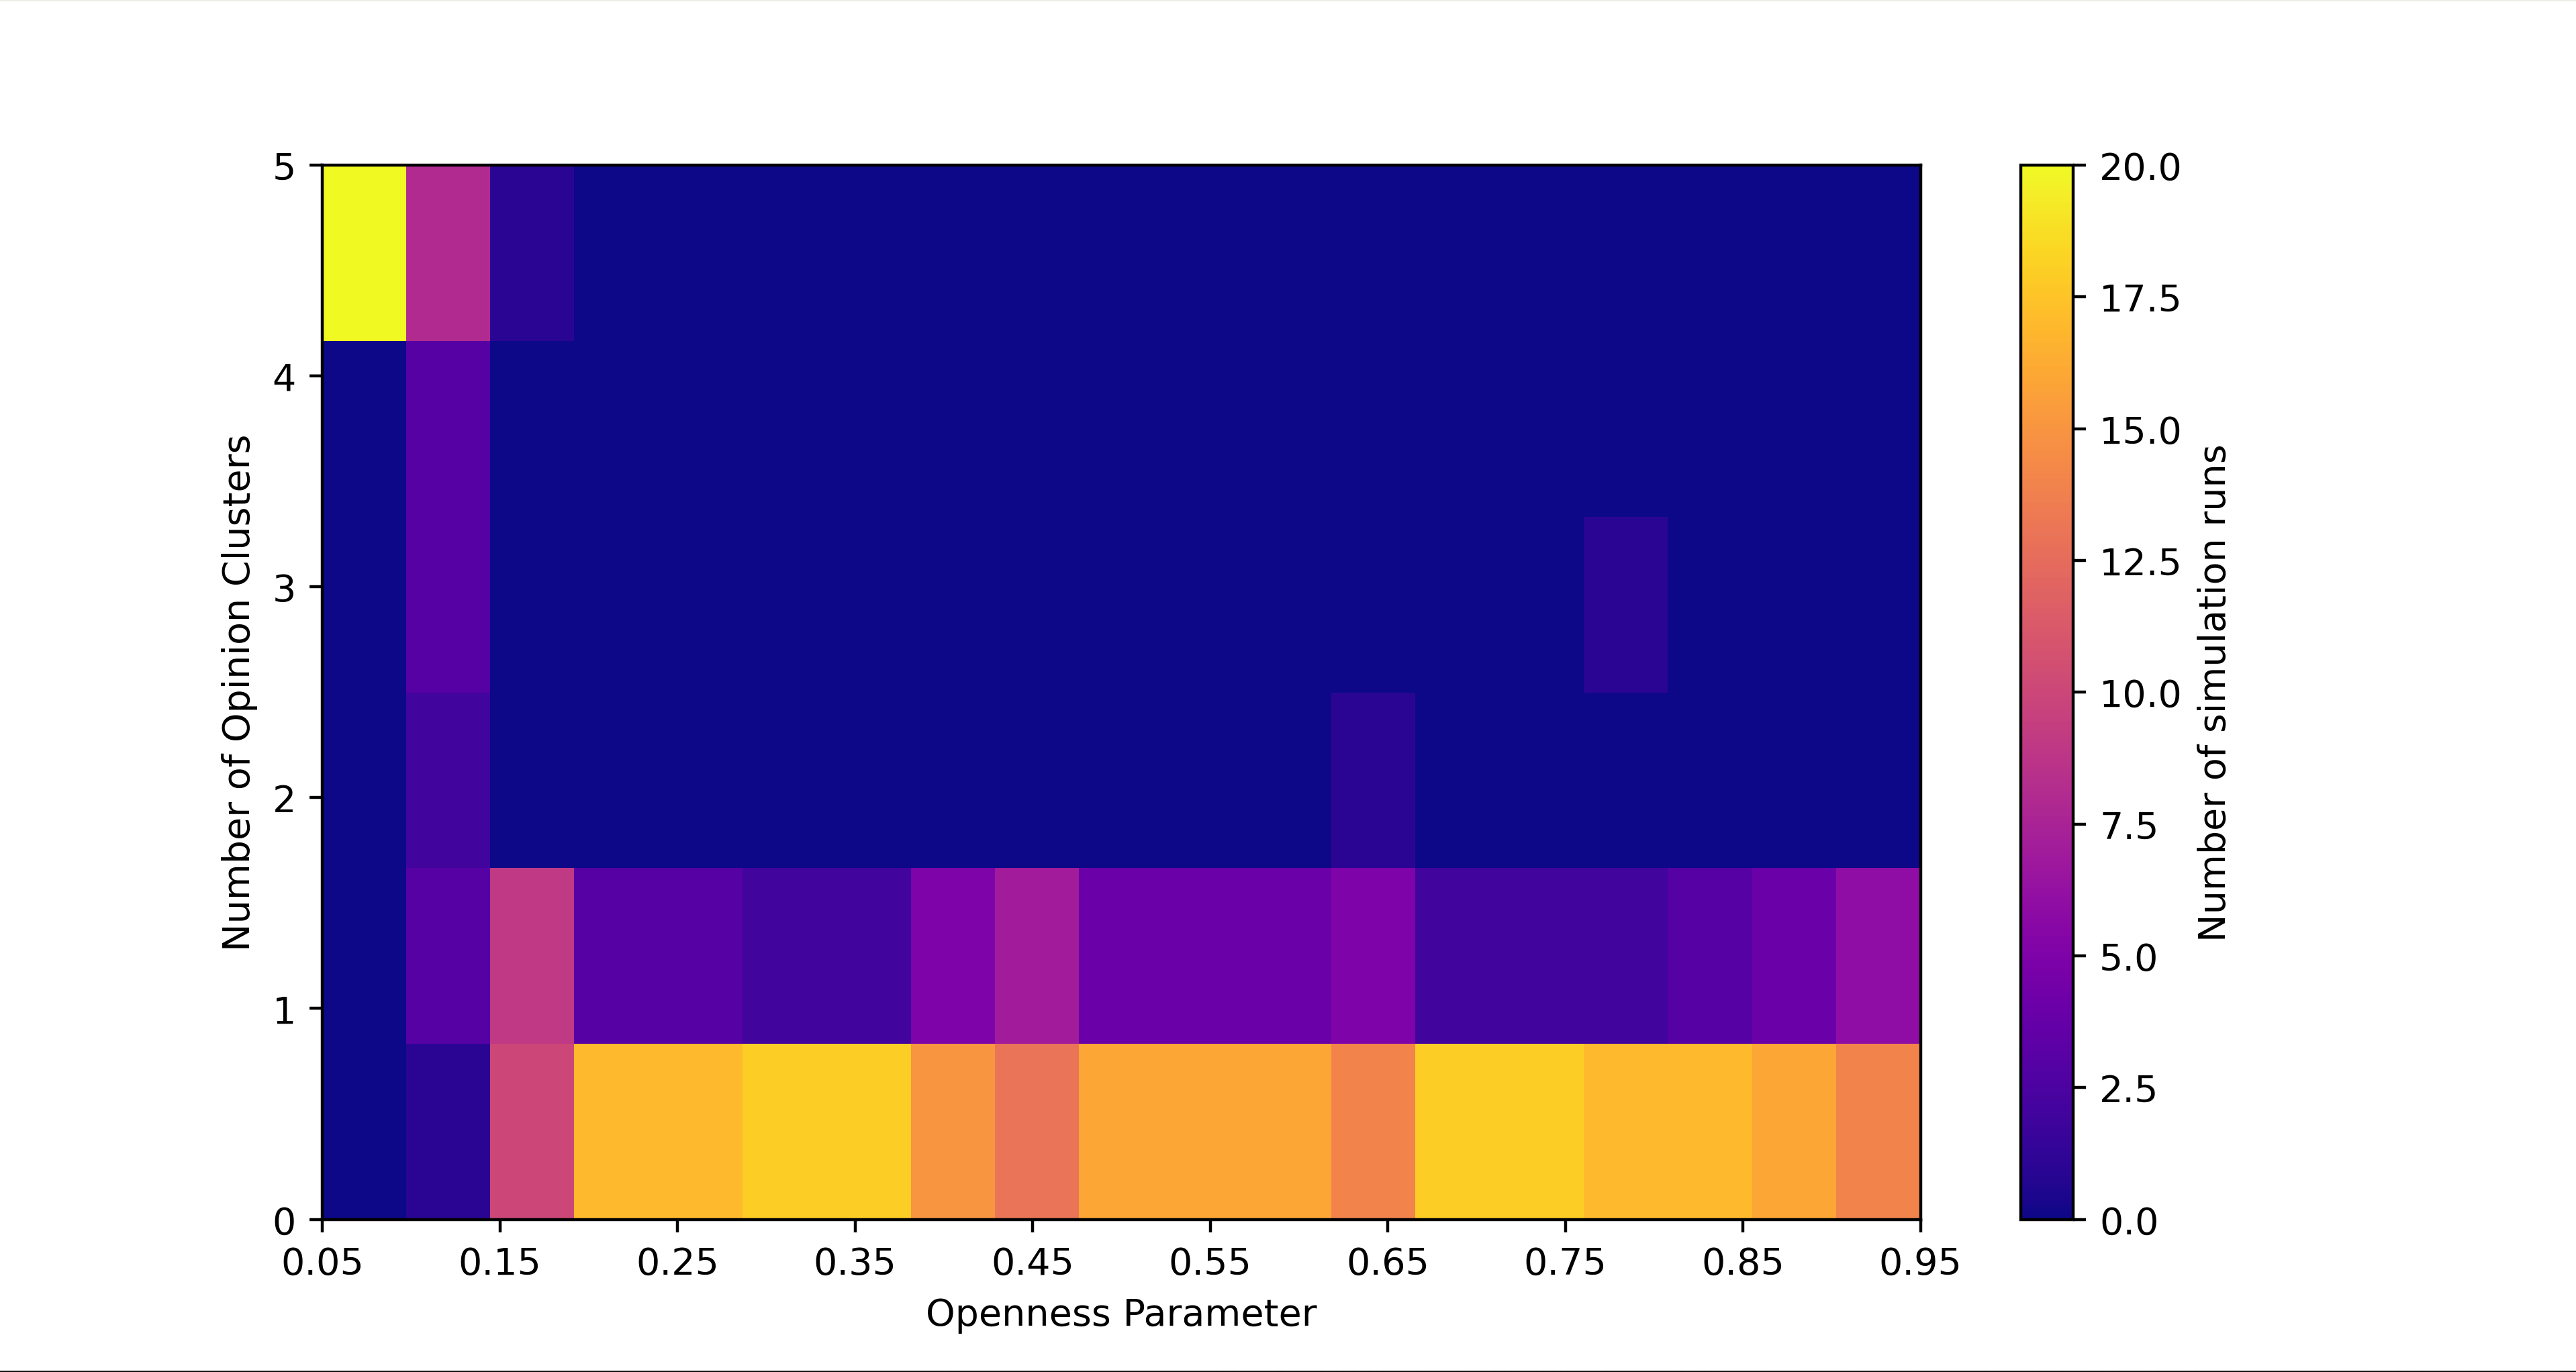
\includegraphics[width=1.0\columnwidth]{./Graphs/Cluster_openBig.png}
\caption{Number of Opinion Clusters and the Openness Parameter (0.05 - 0.95)}
\label{H2b_plot_big}
\end{figure}

We noticed that there was little to no difference between an openness parameter
of 0.5 and 0.7. However, we observed that the openness parameter had more
impact on the number of opinion clusters when the parameter was closer to 0.10.
To further explore this result, we ran another parameter sweep with 50 agents,
5 issues, an edge probability of 0.50, and a suite size of 20. This time, we
varied the openness parameter from 0.05 to 0.40. Our results are depicted in
Figure~\ref{H2b_plot_small}.

\begin{figure}
\centering
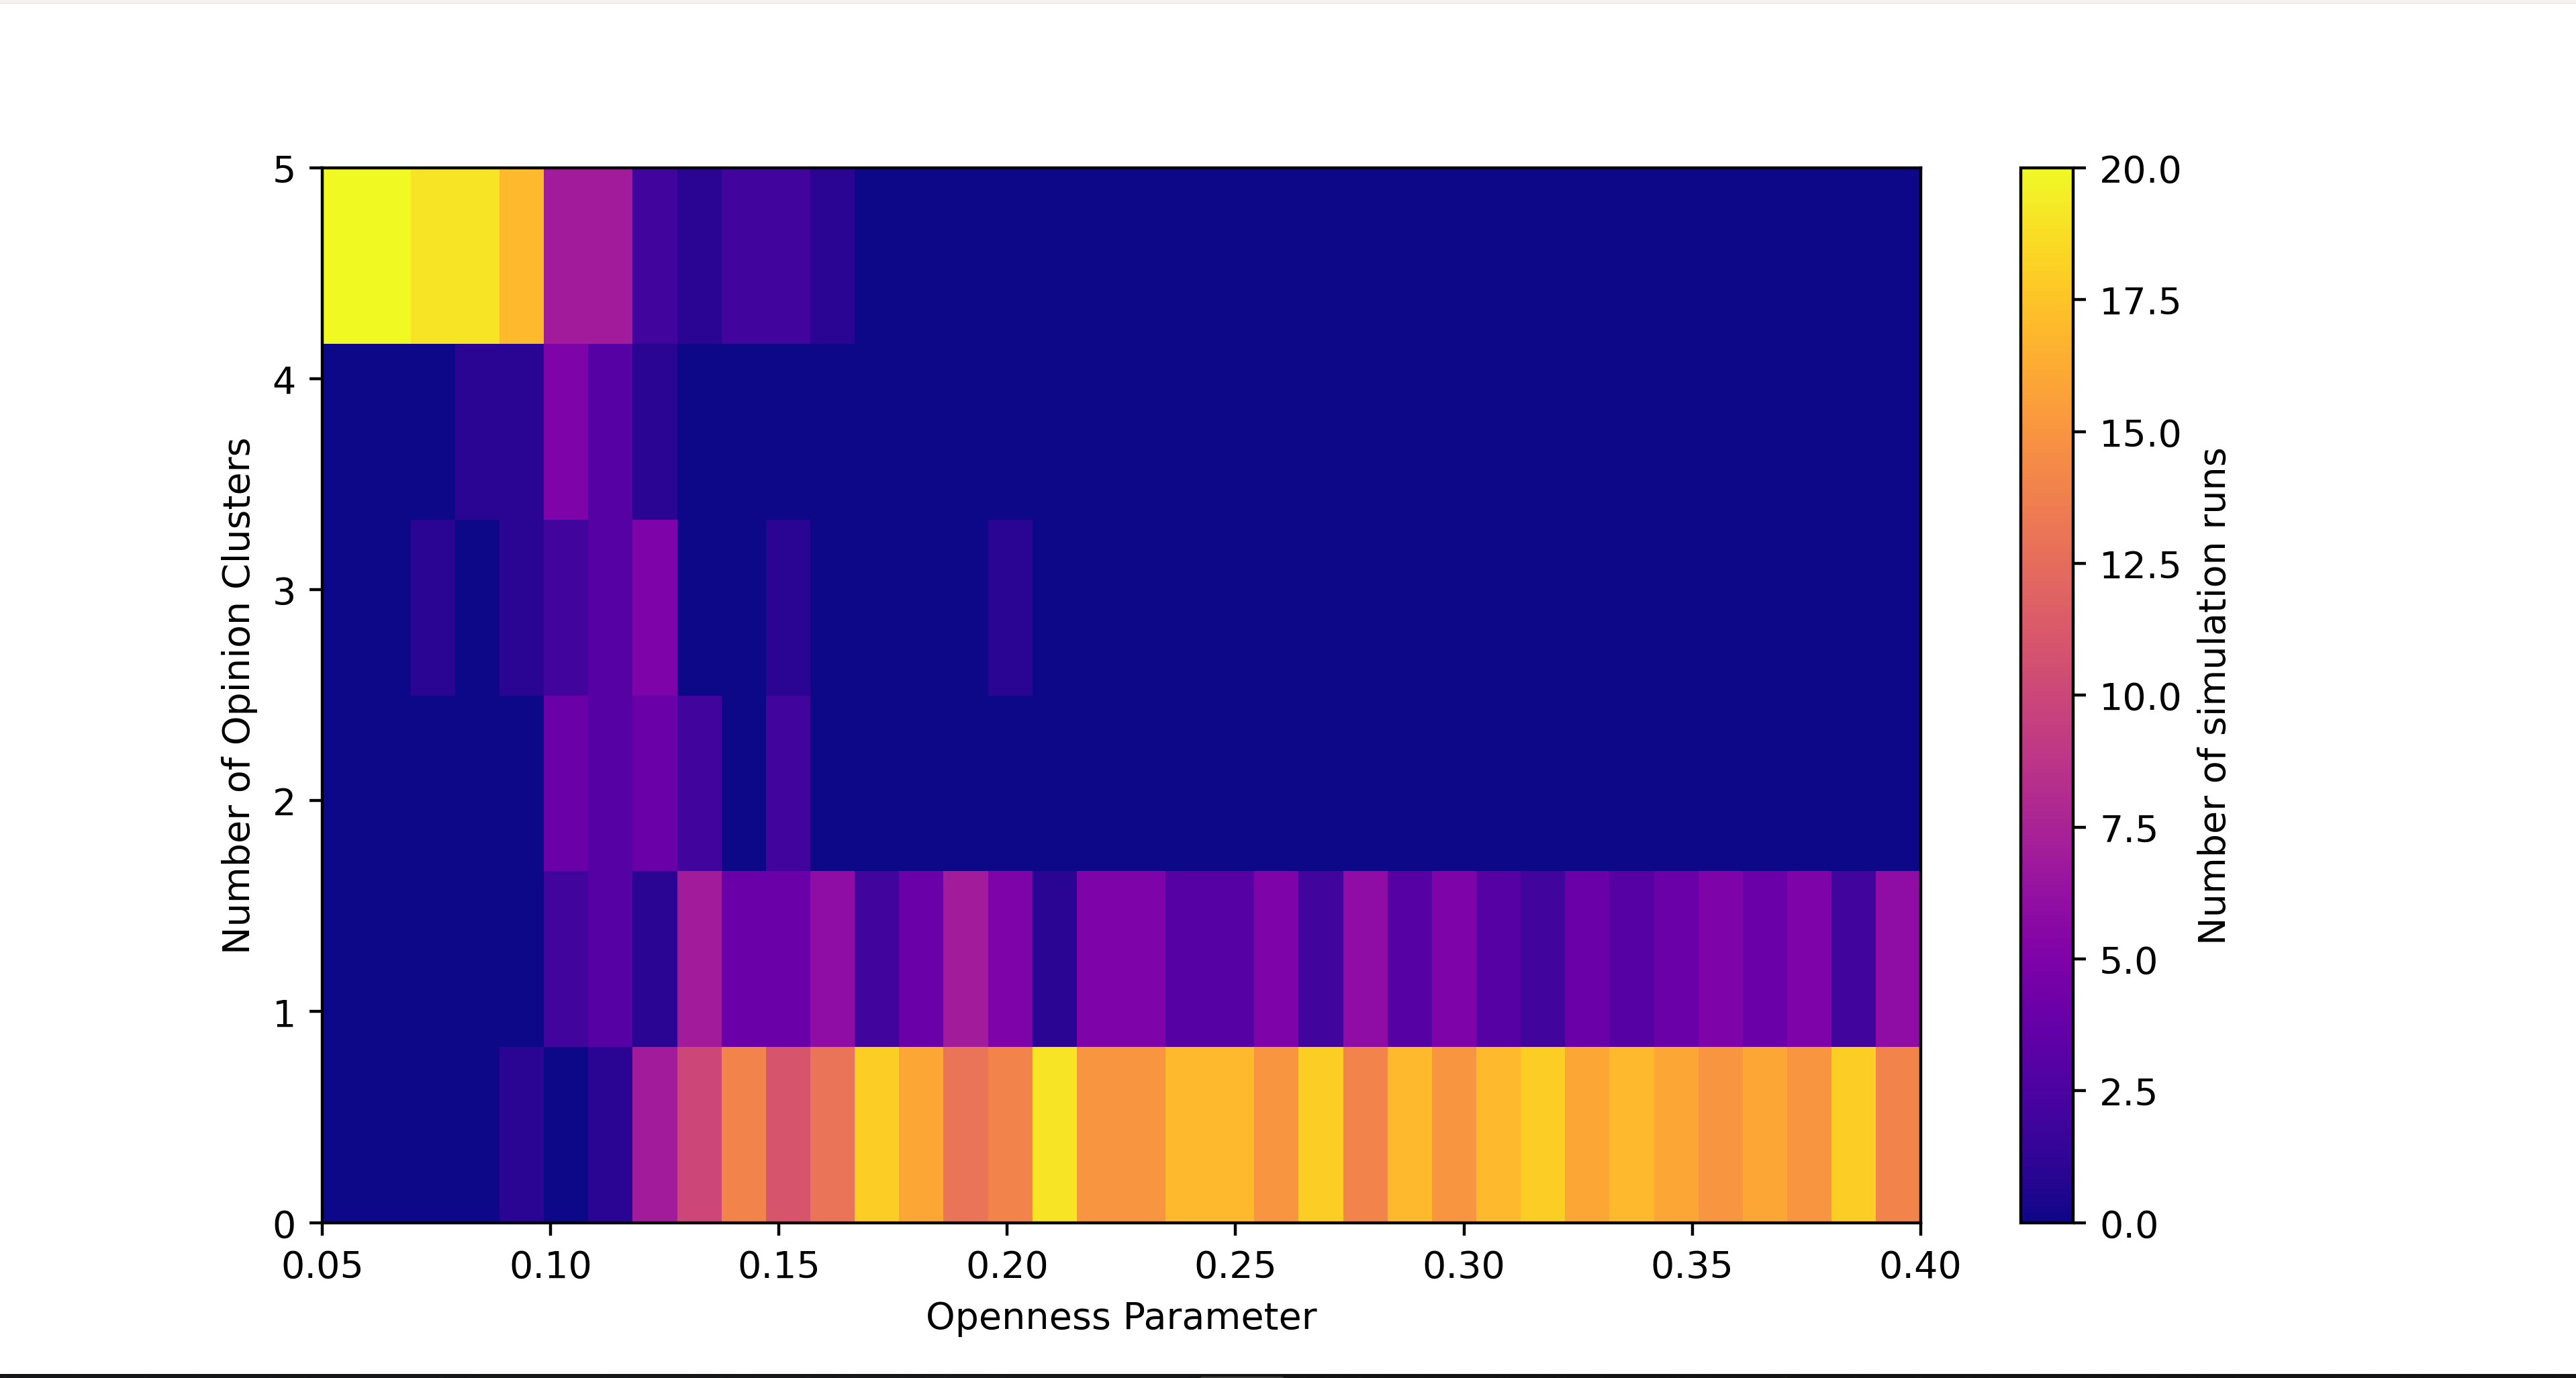
\includegraphics[width=1.0\columnwidth]{./Graphs/Cluster_opensmall.png}
\caption{Number of Opinion Clusters and Openness (0.05 - 0.40)}
\label{H2b_plot_small}
\end{figure}

This graph indicates that there is a tipping point for the openness parameter.
When the openness for agents in the model is very low, the agents did not agree
on many issues. However, as Figure~\ref{H2b_plot_small} indicates, when we
increase the openness parameter slightly, the number of opinion clusters across
the model quickly drops. As a result, we can infer that low levels of openness
in a society may induce more polarized societies. When agents in the model are
less open to distant opinions, there are more opinion clusters for any given
issue. However, the tipping point leads us to believe that slightly higher
levels of openness are sufficient to reach uniformity on a given issue for all
agents in the model. To conclude, when using the cross-issue influence
mechanism, marginally higher levels of openness led to to less polarization in
the model.


\section{Discussion and Future Work}

Multiple results in this research surprised me. Firstly, the results from
testing $H_{1a}$ did not reflect my anecdotal experiences. When increasing the
density of a society's connection, I instead saw \textit{lower} assortativity.
I believe this may be due to the static nature of the model's social network.
In the real world, homophily not only causes existing friends to become more
like each other, but also causes people to select (or reject) friends based on
their similarity. In future work, I intend to add this feature to the model,
producing a dynamic graph, and discover whether this addition is sufficient to
produce a positive density/assortativity relationship.

The lack of a relationship for $H_{1b}$ was another surprising result. I
extensively tested this hypothesis, but the results did not indicate any
statistically significant relationship. This result remains unexplained.

The tipping points observed when testing hypotheses $H_{2a}$ and $H_{2b}$ were
compelling results. When even slightly increasing the density of a graph, the
number of clustered issues can drop quickly. This would seem to indicate that
the degree to which a society forms consensus can be quite sensitive to the
average number of social connections people maintain, at least within a certain
range. Too, the openness of a society's members -- however that might be
quantified in a real population -- produced an even steeper tipping point. One
interpretation would be that even small changes in the tolerance people have
for dissenting views can produce great gains in reducing polarization. I also
plan to investigate the behavior of models with agents that are heterogeneous 
with respect to openness, since OE and other traits are obviously not uniform
across a real population.

Finally, the most exciting results in my opinion were the findings of hypothesis $H_{3}$. This result could have wide-reaching implications on how we interpret the causes of the polarization phenomenon, and what societal changes might be necessary to reduce it. First, this finding shows that neither ideological coherence nor media influence is necessary for issue alignment to develop in a society. It shows that the cross-issue influence mechanism is sufficient. Secondly, issue alignment endogenously appears through the CI2 mechanism. The model was not initialized with any interdependencies between issues, yet this phenomenon develops consistently through CI2. 

Although this is an exciting result, it is hard to be joyful about replicating a negative phenomenon such as polarization. However, replicating polarization has left me with certain ideas about how to reduce polarization from the individual and societal perspective. First, relating to the finding that lower network density leads to higher polarization, I believe that a potential fix for individuals is to surround yourself with more people. By increasing your number of social connections, there is a higher chance you will be exposed to a more diverse set of opinions; thus, lowering your chance of being in an echo chamber. Second, relating to the openness findings, I believe that individuals can help to reduce societal polarization by increasing their tolerance level to dissenting opinions. Finally, relating to the issue alignment findings from $H_{3}$, I believe the solution is to allow yourself the freedom to agree with someone on one thing and disagree with them on something else. By keeping unrelated issues separate, the cross-issue influence mechanism can be reduced which would decrease the degree of issue alignment in society. From a societal perspective, to reduce the issue alignment we need voices from more buckets. The two party system and global media outlets undoubtedly reinforce the issue alignment phenomenon. The solution on a macro level is larger variety of reasonable opinions.    


\appendix

\bibliographystyle{ACM-Reference-Format}
\bibliography{mitterederEtAl}
\end{document}
